\chapter{Nanopore Signal Analysis}
\label{cha:signal}

The primary output of third generation nanopore sequencing devices is the measured raw ionic current as a proxy signal for a DNA or RNA strand passing through the pore. 
An initial processing step of particular importance is the basecalling, translating the raw signal into the respective genomic sequence.
Common workflows such as genome assembly, structural variant or isoform detection typically rely on sequence inputs only.
However, the error rate and run time of state of the art basecalling algorithms motivate ongoing research on the processing of the raw signal itself. Furthermore, the sequencing without amplification preserves signatures of modified bases in the signal of DNA and RNA samples.
Prominent applications based on raw nanopore signals include methylation detection, barcode demultiplexing and real-time alignment for selective sequencing.
Challenges in the raw signal analysis arise from noise induced by measuring currents in pico ampere ranges and time-warping, the uncertainty of how long the molecule resides stationary in the pore before being advanced by the motor protein.


\begin{figure}[h]
    \centering
    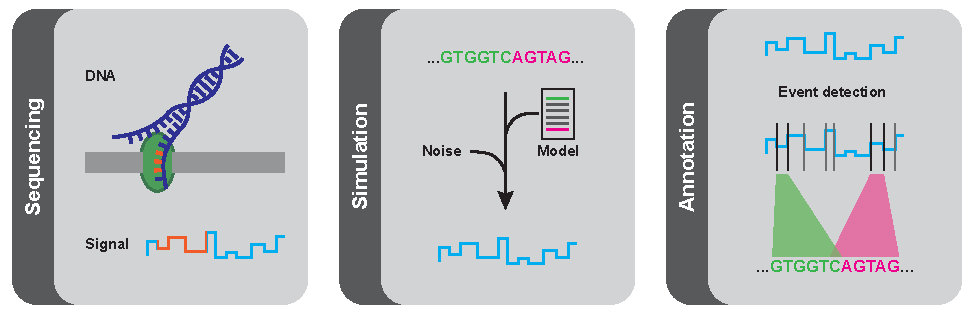
\includegraphics[width=1.0\textwidth]{figures/signal/GA.pdf}
    \label{fig:signal:ga}
\end{figure}


The following chapter serves as a transition from basic data handling and processing using \textit{Nanopype} in chapter \ref{cha:nanopype} and introduces the underlying algorithms for the signal driven repeat detection \textit{STRique} in chapter \ref{cha:strique}.
After a brief \textbf{background} in section \ref{sec:signal:background}, this chapter covers the raw signal \textbf{simulation} from known sequences in section \ref{sec:signal:simulation} and the \textbf{normalization} and \textbf{annotation} of raw nanopore reads with reference sequences in sections \ref{sec:signal:normalization} and \ref{sec:signal:alignment}.

\section{Background}
\label{sec:signal:background}

In contrast to second generation sequencing, the main output of nanopore sequencing is the ionic current measured on the device while a molecule is passing through any of its pores. The characteristics of this signal are determined by pore and chemistry version, currently R9.4.1, as released by ONT in October 2016. In March 2020 ONT released the R10.3 with a dual reader head, promising better consensus accuracy, in particular for homopolymer stretches. In terms of throughput per flow-cell, the R10 is slightly lacking behind R9 \cite{ONT2020}. Independent of the pore version, the storage of the raw signal is valuable, as constant development by ONT and researchers in the community provides enhanced readouts from existing sequencing data.

From a technical perspective, the ionic current is sampled at 4kHz and saved as a 16-Bit unsigned integer array to FAST5 files. In combination with the sequencing speed of \texttildelow450nt/s, determined by the chemistry, this results in a square wave like signal with a median of 9 samples per nucleotide. Being a specification of the HDF5 file format, FAST5 files can be inspected with GUI and command line tools like \textit{HDFView} and \textit{h5dump}. File access from custom software is available for C/C++ programs by linking against the HDF5 library\footnote{https://bitbucket.hdfgroup.org/projects/HDFFV/repos/hdf5/browse} and from python using the \textit{h5py} package. Additionally, in order to work with most recent data sets, the VBZ compression plugin\footnote{https://github.com/nanoporetech/vbz\_compression} is required.

While the raw nanopore signal is utilized in a number of bioinformatic applications \cite{Simpson2017, Wick2018, Loose2016}, the set of methods providing frameworks is currently limited to \textit{Tombo}\footnote{https://github.com/nanoporetech/tombo}, the successor of \textit{Nanoraw} \cite{Stoiber2017} and the recently published \textit{SquiggleKit} \cite{Ferguson2019}. The motivation to develop and use custom code for the raw signal analysis is driven by \textit{Tombo} being hard-coded to \textit{minimap2} alignments and writing its output in form of event tables into the FAST5 files. While technically supported by the FAST5 format, writing of analysis results into the sequencing data is generally undesirable in a multi-user environment and causes in the case of FAST5 files excessive disk usage since new, but also overwritten data sets are appended to the end of the file. \textit{SquiggleKit} so far only provides basic data indexing and signal alignment, mostly to identify barcodes in raw reads.

Publicly available, highly customizable methods in form of a generic API are still lacking, demanding the development of an in-house framework to handle raw nanopore reads. Future work aims to include advanced normalization methods as described in \cite{Boza2017} and hardware acceleration comparable to \textit{f5c} \cite{Gamaarachchi2020}.




\section{Simulation}
\label{sec:signal:simulation}

Third generation sequencing data can be simulated on different levels, by generating sequences with realistic read length and error rate distributions or by generating raw signal traces, ideally indistinguishable from measured ones. Simulated reads of both types are helpful to develop or test applications under controlled conditions. Two state of the art simulators are \textit{simulatION} \cite{Rohrandt2018} and \textit{deepSimulator} \cite{Li2020}, following different concepts to generate FAST5 files of simulated reads, which can be processed with common workflows. While the former utilizes exiting models of level and noise, the latter uses a LSTM neural network to generate the signal from reference sequences. Nonetheless, generation of realistic signal traces in memory can already be achieved with a pore model and an event length distribution.

A pore model describes the mapping from sequence context to expected signal level. The ionic current in the nanopore is determined by the local sequence context termed kmer. Current models utilized by e.g. \textit{nanopolish} contain mean and standard deviation of signal levels per 6mer. The distribution of all, in this case 4096 levels is shown in Fig. \ref{fig:signal:pm} a, emphasizing the multi-modal characteristic of the R9.4 pore.

\begin{figure}[h]
	\centering
	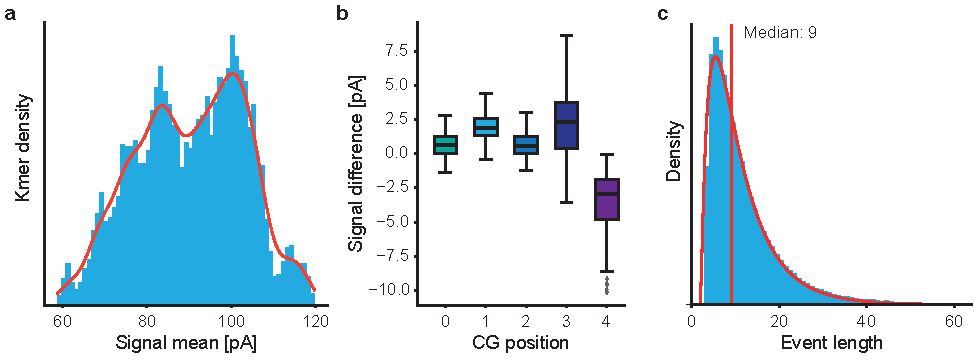
\includegraphics[width=1.0\textwidth]{figures/signal/pm.pdf}
	\captionsetup{format=plain}
	\caption[Pore model and event length]{Pore model and event lengths: \textbf{a}, Density plot and kernel density estimation of expected signal levels per kmer (k=6, n=4096, mean ionic current in pA). \textbf{b}, Expected signal difference of native and 5mC modified DNA for 6mers with single CG (n=256 per position) depending on the CG location. \textbf{c}, Event length (samples per kmer) density plot from signal alignment (red: approximation by generalized gamma distribution with a=4.3, c=0.6, shit=2, scale=0.7).}
	\label{fig:signal:pm}
\end{figure}

In general, the nanopore is sensitive for several base modifications, which are preserved when sequencing without prior amplification. A secondary pore model can be derived from sequencing e.g. 5-methylcytosine modified DNA, enabling the discrimination of native and 5mC on signal level. The model difference between native and 5mC for single-CG containing 6mers is illustrated in Fig. \ref{fig:signal:pm} b (Native and methylated model taken from \textit{nanopolish}).

In addition to the signal level, the event length or dwell time of the molecule in the pore needs to be modeled. It is not fully understood, to which extend the behavior of the motor protein controlling the sequencing speed is a random or sequence context dependent process. Aimed solely towards the development of signal alignment methods, event lengths are randomly sampled from a generalized gamma distribution in this work. 
The distribution is derived from in-house sequencing data using the event detection described in section \ref{sec:signal:alignment} and shown in Fig. \ref{fig:signal:pm} c. The measured event median of 9 samples per 6mer matches the expected value for a sequencing speed of 450nt/s sampled at 4kHz.

With both, pore model and event length distribution, simulated raw nanopore signals can be generated from any given target sequence. The mean event level, a simulated and the corresponding stretch from a real nanopore read are depicted in Fig. \ref{fig:signal:simulation}.

\begin{figure}[h]
	\centering
	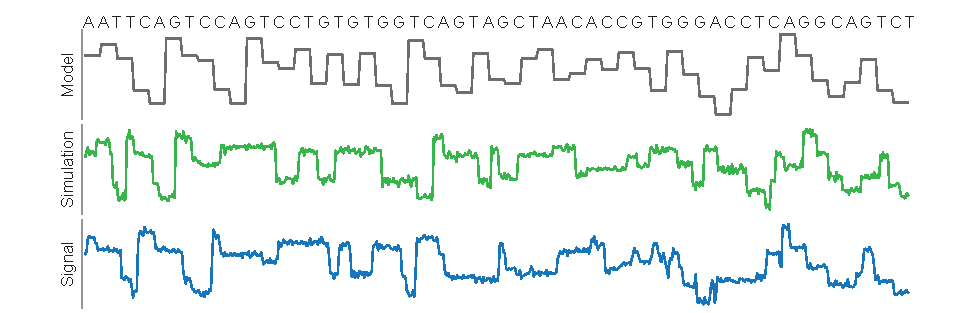
\includegraphics[width=1.0\textwidth]{figures/signal/simulation.pdf}
	\captionsetup{format=plain}
	\caption[Basic signal simulation]{Basic nanopore signal simulation from pore model and event lengths: Mean ionic current levels per kmer for short sequence (top), simulated nanopore signal with noise and random time warping (center) and raw signal fragment extracted from real nanopore read covering the same sequence (bottom).}
	\label{fig:signal:simulation}
\end{figure}

Published and the proposed simplified simulation do not mirror every detail of actual sequencing data and can therefore only serve as a first approximation. Examples of missing technical artifacts are rare spikes of single values and temporarily stalled reads with hundreds of samples from the same kmer. Lastly, motor protein and analog digital converter are not synchronized, frequently resulting in measurements on the rising or falling edges between events.




\section{Normalization}
\label{sec:signal:normalization}

A robust normalization is a substantial first step during nanopore signal processing, impacting any downstream method and readout. Baseline for the following normalization is the raw ionic current measurement, saved by the sequencing software \textit{MinKNOW} as unmodified unsigned integer with a typical numeric range from 300 to 700 (cf. Fig. \ref{fig:signal:normalization} top track). Prior to any processing in this work we apply a median filter with a sliding window of length three to remove signal spikes and reduce the overall noise. Factors affecting the signal levels are:

\begin{itemize}
	\item Individual offset and scale induced by the electronic circuit per pore
	\item Uneven sequence composition depending on the genomic context resulting in biased sampling from the multi modal pore model
\end{itemize}

Offset and scale for normal distributed signals can be compensated by using a straightforward z-score normalization:

\begin{equation}
	X_{norm,zscore} = \frac{X_{i} - \mu}{\sigma}
\end{equation}

Suggested by \textit{Nanoraw} \cite{Stoiber2017} and more robust against the underlying distribution is a median normalization defined as:

\begin{equation}
	X_{norm,median} = \frac{X_{i} - median(X)}{median(\left|X_{i}-median(X)\right|)}
\end{equation}

With regard to the signal driven repeat quantification in chapter \ref{cha:strique}, we propose a novel strategy combining a min-max and quantile normalization. Subtraction of the signals 0.025 quantile and scaling by its interquantile range appears to be more robust against outlier and biased signal distributions:

\begin{equation}
	X_{norm} = \frac{2 \cdot (X_{i} - Q_{0.025})}{Q_{0.975} - Q_{0.025}} - 1
\end{equation}

The min-max normalized signal with most values in the range $ [-1:1] $ maintains the characteristics of the nanopore, is comparable to simulated reads using a pore model and in this form used for the repeat quantification in chapter \ref{cha:strique}.

For the purpose of signal alignment and event segmentation we propose two additional steps of  histogram equalization and morphological smoothing \cite{Gonzalez2006}. Commonly used to enhance the contrast of digital images, a histogram equalization can be used to project the multi-modal distribution of mean event levels (Fig. \ref{fig:signal:pm} a) to a more uniform distribution (Fig. \ref{fig:signal:normalization} bottom track). 

To further reconstruct the expected square wave like signal, we apply a morphological noise removal, specifically an opening followed by a closing with a structuring element of length three.

\begin{figure}[h]
	\centering
	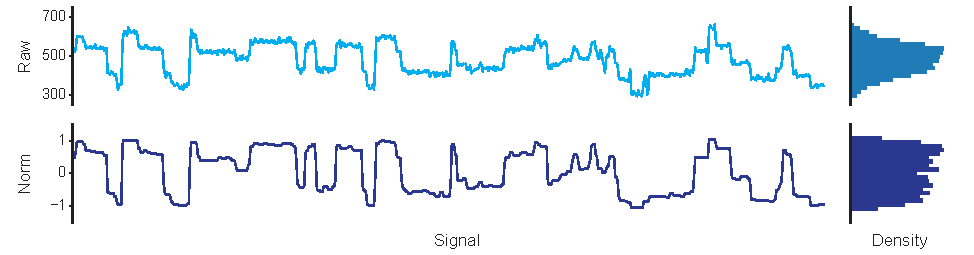
\includegraphics[width=1.0\textwidth]{figures/signal/normalization.pdf}
	\captionsetup{format=plain}
	\caption[Signal normalization and histogram equalization]{Signal normalization and histogram equalization followed by morphological noise reduction on raw nanopore signal traces. The figure shows signal segments over a 50nt window in combination with density plots of raw and normalized values over the entire read.}
	\label{fig:signal:normalization}
\end{figure}

The final result of normalized and filtered signal with a near uniform distribution of values across the full signal range is the baseline for the alignment and event detection described in the following section.




\section{Segmentation and Alignment}
\label{sec:signal:alignment}

For applications, where neither signal nor sequence alone enable the intended readout, the sample wise annotation of raw signals with the respective reference sequence is required. Affected by the basecalling error of around 5-10\% (cf. Fig. \ref{fig:state_of_art:throughput} b), the usage of the reference sequence after read alignment is preferable over the read sequence.

Primarily to extract larger regions of interest from a raw signal, we specify a template function of the \textit{SeqAn2} \cite{Reinert2017} library to perform a distance based semi-global signal alignment. Specifically, we utilize the \textit{globalAlignment} function with a float32 data type, an affine gap penalty and the following score function:

\begin{equation}
s_{i,j} = max \left\lbrace c - \left| x_{i} - y_{j} \right| \atop 0 \right.
\end{equation}

The alignment is executed between the normalized raw signal and a simulated signal with constant event length of either complete reference span or a query region of interest within the read.
The absolute signal difference per position is translated into a score by subtracting it from a constant \textit{c}. The score is capped at zero as lower boundary, resulting in a fixed minimum mismatch score independent of the actual signal difference.
Gap costs within signal and simulation are configured differently. Both, gap open and gap extension penalty in the signal are set to -0.1 with the begin and end gaps being free (semi global alignment). Gaps in the simulated reference signal are penalized with -1.6 for open and extension. 
The rationale behind is that gaps in the signal are expected and introduced by simulated single value events being stretched to the observed lengths. Gaps in the simulated reference signal are expected to by very rare and stand for sequence stretches not being observed in the raw signal.





symbolization paper \cite{Lin2003}

\begin{table}[ht]
	\centering
	\caption[Event detection and annotation]{Event table of raw nanopore signal with reference sequence annotation.}
	\label{tab:signal:events}
	\begin{tabular}{l|r|r|r|l}
		 & mean & event length & seq. offset & kmer \\
		\hline 
		& \multicolumn{3}{c|}{...} &  \\
		\hline
		$ E_{n} $ &  1.332  & 15 & 3205 & AGTCCA \\
		\rowcolor{LightOrange}
		$ E_{n+1} $ &  0.981  & 22 & 3206 & GTCCAG \\
		$ E_{n+2} $ & -1.058  &  6 & 3208 & CCAGTC \\
		$ E_{n+3} $ & -1.662  & 17 & 3209 & CAGTCC \\
		$ E_{n+4} $ &  1.360  &  7 & 3210 & AGTCCT \\
		$ E_{n+5} $ &  0.664  & 33 & 3211 & GTCCTG \\
		$ E_{n+6} $ &  0.107  & 11 & 3212 & TCCTGT \\
		\rowcolor{LightGreen}
		$ E_{n+7} $ &  0.844  &  4 & 3213 & CCTGTG \\
		\rowcolor{LightGreen}
		$ E_{n+8} $ &  1.362  & 38 & 3213 & CCTGTG \\
		\hline
		& \multicolumn{3}{c|}{...} &  \\
	\end{tabular} 
\end{table}


\cite{Schreiber2015}

\begin{figure}[h]
	\centering
	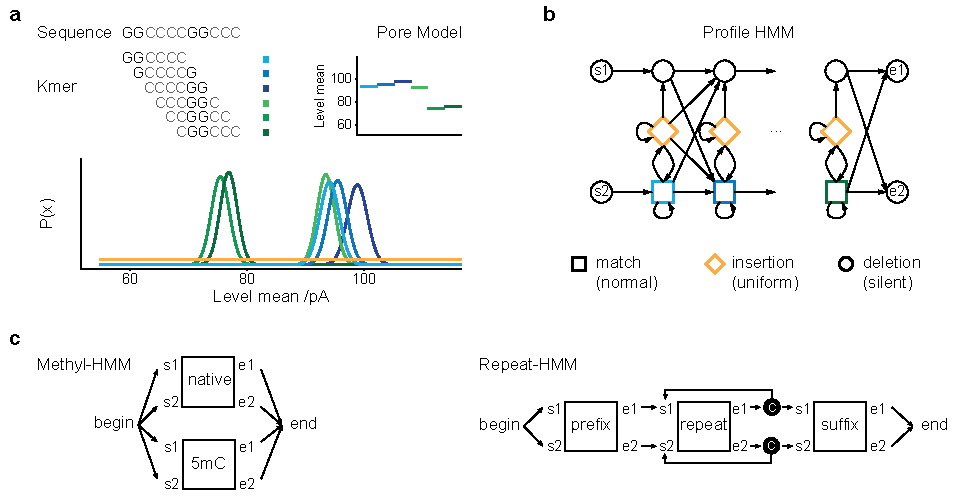
\includegraphics[width=1.0\textwidth]{figures/signal/count_hmm.pdf}
	\captionsetup{format=plain}
	\caption[Nanopore signal alignment with HMMs]{\textbf{a}, A compound profile HMM of prefix, a single repeat and the suffix sequence assigns either prefix, repeat or suffix label to each signal value. Repeat counts are obtained through dummy states between repeat and suffix. \textbf{b}, Nanopore signal profile HMM with normal distributed match state and uniform distributed insertion state emission probabilities.}
	\label{fig:strique:count_hmm}
\end{figure}


\begin{itemize}
	\item raw signal alignment with seqan based scoring and semi-global dp
	\item segmentation with basic image processing tools, edge filter + threshold
	\item event alignment with edlib to be more robust against time-warping
	\item profile HMM for most precise mapping
\end{itemize}

\section{Summary}
\label{sec:signal:summary}



